\Chapter{JavaScript implementáció}

\Section{A kliens program működése}

\begin{figure}[h]
\centering
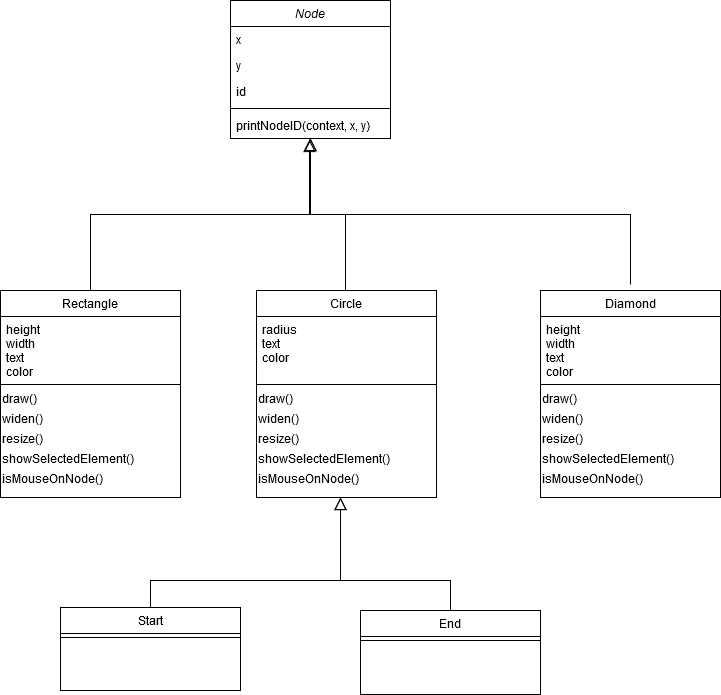
\includegraphics[scale=0.5]{images/umldiagram.png}
\caption{A program UML diagramja}
\label{fig:uml}
\end{figure}

A kliens program a következőképpen működik: A graphEditor.html dokumentum betöltése után létrehozzuk az Editor osztály egy példányát. Ezután inicializáljuk a szerkesztőt egy függvény segítségével. Itt beállítjuk a program működéséhez elengedhetetlen adattagokat, események kezelését. Ilyen adattagok a graph, canvas, context, themes.

Végül egy metódus segítségével átméretezzük az adott böngészőablak méretéhez arányosra a canvas-t, biztosítva így, hogy bármilyen méretű képernyőn használható legyen a program.

Az indítás után a program egy aszinkron GET kéréssel lekéri az adatokat a szervertől JSON formátumban. Az adatokból létrehozza a megfelelő osztályokat a konstruktor paraméterekkel. Ezután a csomópontokat hozzáadja a nodes adattaghoz.

\begin{javascript}
function GetEditorData() {
   fetch(apiURL+'/nodes').then(response => response.json())
       .then(data => {
           console.log(data);
           data.map(node => {
               let newNode = {};
               switch (node["type"]) {
                   case "rectangle":
                       newNode = new Rectangle(node["x"],node["y"],node["id"],node["height"], node["width"], node["text"], editor.graph.themes[editor.graph.selectedtheme].rectangleColor);
                       break;
                   case "circle":
                       newNode = new Circle(node["x"],node["y"],node["id"],node["radius"], node["text"], editor.graph.themes[editor.graph.selectedtheme].circleColor);
                       break;
		//...a tobbi csomopontra hasonlokeppen
               }
               let index = editor.graph.nodes.push(newNode) -1;
               editor.graph.selectedIndex = index;
               editor.addTextToNode(node["text"]);
           })
\end{javascript}

Ha ez sikerült, a függvény egy Promise-szal (ígéret) jelzi, és lekérhetjük az összekötő vonalakat. Mivel aszinkron az előző kérés is, előfordulhat olyan, hogy az összekötő vonalak hamarabb megérkeznek, mint maguk a csomópontok, és ez a programban végzetes hibához vezetne. Ezért van szükség a Promise-ra. 

\begin{javascript}
       .then(r => {
           //itt mar betoltottuk a nodes-okat
\end{javascript}

Ezután egy másik GET kéréssel lekérjük az összekötő vonalakat, és a megfelelő adatokból létrehozzuk az Edge osztály példányait, és hozzáadjuk őket az edges adattaghoz, így a következő rajzolásnál már látszódnak a gráfok. 

A szerkesztő állapotát a következőképpen tudjuk elmenteni: A mentés gombra kattintva először átalakítjuk a nodes és edges adattagokban található osztályokat JSON adattá, majd egy aszinkron POST kéréssel mentjük az adatokat a szerveren.

A csomópontokat megvalósító osztályokat univerzálisan kezeljük: amilyen tulajdonsággal nem rendelkeznek, egyszerűen 0-ra állítjuk, úgyse foglalkozunk velük.

\begin{javascript}

       let nodeJSON = {
           "type": type,
           "x": node.x,
           "y": node.y,
           "id": node.id,
           "text":node.text,
           "height": node.height ? node.height : 0,
           "width": node.width ? node.width : 0,
           "radius": node.radius ? node.radius : 0,
           //"theme": editor.graph.selectedtheme
       };
       nodes.push(nodeJSON)
\end{javascript}

Az összekötő vonalakat is csak azután küldjük el a szervernek, hogy megbizonyosodtunk arról, hogy a csomópontokat hibamentesen elmentettük. Az SQLite adatbázisban olyan idegen kulcs relációval kapcsolódnak a vonalak a csomópontokhoz, hogy ha a csomópont nem létezik, nem tudjuk elmenteni az összekötő vonalat.
 
Az eseménykezelés a következőképp zajlik: A billentyűk lenyomásához és felengedéséhez az editor megfelelő metódusát rendeljük.

\begin{javascript}
window.addEventListener("keydown", editor.keyDown, false);
window.addEventListener("keyup", editor.keyUp, false);
editor.graph.canvas.addEventListener("mousedown", editor.mouseDown.bind(editor), false);
editor.graph.canvas.addEventListener("mousemove", editor.mouseMove.bind(editor), true);
editor.graph.canvas.addEventListener("mouseup", editor.mouseUp.bind(editor), false);
editor.graph.canvas.addEventListener("mousewheel", editor.mouseWheel.bind(editor), false);
\end{javascript}
 
Például a \textit{mouseDown} eseménykezelő metódus úgy működik, hogy ha lenyomjuk az egér bal gombját, a függvény újra rajzoltatja a gráfokat, majd kiszámítja, hogy az egér rajta van-e valamely csomóponton. Ha rajta van, az lesz az éppen kijelölt csomópont, és a csomópont osztályban jelez, hogy húzható (\textit{drag}) állapotba került, azaz az éppen kijelölt csomópont követi az egérmutató mozgását.

\begin{javascript}
mouseDown(event)
{
   this.graph.clear();
   this.graph.draw();
   const mouse = this.calcMouseEvent(event);
   this.graph.selectedIndex = null;
   for (let i = 0; i < this.graph.nodes.length; ++i) {
       let node = this.graph.nodes[i];
       if (node.isMouseOnNode(mouse['x'], mouse['y'])){
           this.graph.selectedIndex = i;
       }
   }
   this.graph.dragStart = {
       x: event.clientX - this.graph.canvasPosition.left,
       y: event.clientY - this.graph.canvasPosition.top
   };
   this.graph.drag = true;
}
\end{javascript}

 
Ha a megfelelő helyre húztuk a csomópontot, és felengedtük az egér bal gombját, a \textit{mouseUp} eseménykezelő metódus jelzi a csomópontokat kezelő osztálynak, hogy a csomópont már nem húzható, azaz nem követi tovább az egeret.

\begin{javascript}
mouseUp(event, context)
{
   this.graph.clear();
   this.graph.draw();
   const mouse = this.calcMouseEvent(event);
   this.graph.drag = false;
}
\end{javascript}

A csomópontokat úgy tudjuk összekötni, hogy a kiinduló (forrás) csomópontra rákattintunk, miközben nyomva tartjuk a \texttt{Shift} billentyűt. Egy másik (cél)csomópontra kattintva, miközben nyomva tartjuk az \texttt{Alt} billentyűt, kijelölhetjük az összekötendő csomópontot. A \texttt{Ctrl} billentyűvel, és bal egér kattintással törölni tudjuk a csomópontot.

Vonalat törölni szintén a Shift és a Alt billentyűk segítségével lehet (úgy, mint a létrehozásnál), itt viszont a jobb egérgombot kell lenyomnunk a billentyűk mellé.

Ezek között az \texttt{event.which} száma tesz különbséget: Az 1-es a bal egérgombra vonatkozik, a 3-as pedig a jobbra.

\begin{javascript}
if (event.shiftKey === true) {
    this.graph.drawEdge['from'] = this.graph.nodes[selectedIndex];
}
if (event.altKey === true) {
    this.graph.drawEdge["to"] = this.graph.nodes[selectedIndex];
    if (event.which === 1 ){
        //node["id"];
        this.addEdge(this.graph.drawEdge["from"], this.graph.drawEdge["to"]);
        this.graph.clear();
        this.graph.draw();
    } else if (event.which === 3){
        for (let j = 0; j < this.graph.edges.length; ++j) {
            if(this.graph.nodes[selectedIndex] === this.graph.edges[j].to)
            {
                this.graph.edges.splice(j, 1);
                j = j-1;
                this.graph.clear();
                this.graph.draw();
            }
        }
    }

}
if (event.ctrlKey === true) {
    for (let j = 0; j < this.graph.edges.length; ++j) {
        if(this.graph.nodes[selectedIndex] === this.graph.edges[j].to || this.graph.nodes[selectedIndex] === this.graph.edges[j].from)
        {
            this.graph.edges.splice(j, 1);
            j = j-1;
        }
    }
    this.graph.nodes.splice(selectedIndex, 1);
    this.graph.clear();
    this.graph.draw();
}
\end{javascript}

Az automatikus és manuális méretnövelés a következőképpen működik: Minden csomópontnak van megfelelő metódusa a feladathoz, ami a csomópont saját tulajdonsága alapján elvégzi a feladatot. Például a \textit{widen(length)} metódus elfogad egy paramétert, amely ha túl nagynak bizonyul, növeli a csomópont méretét. A téglalap esetében a szélességet növeljük:

\begin{javascript}
widen(length){
   if(15 > (this.width/length))
   {
       this.width = parseInt(this.width) + 14;
   }
}
\end{javascript}

Viszont például egy körnél a sugarat növeljük:

\begin{javascript}
widen(length){
   if(8 > this.radius / length)
   {
       this.radius += 7;
   }
}
\end{javascript}

Átméretezni egy csomópontot a \textit{resize()} metódussal lehet, itt is hasonlóan a csomópont tulajdonságaihoz megfelelő logikával:

\begin{javascript}
resize(){
   this["width"] = parseInt(document.getElementById("width").value);
   this["height"] =  parseInt(document.getElementById("height").value);
}
\end{javascript}
\Section{Felhasználói kézikönyv a programhoz}

Ez az alfejezet írja le a már korábban többször is említett konkrét kezelését az elkészült gráf szerkesztőnek.

\SubSection{Csomópont hozzáadása}

A bal oldali eszköztárban rákattintunk a hozzáadandó elemre, így az megjelenik a szerkesztő felületen egy előre definiált helyen. Ezt követően az adott csomóponton a bal egérgombot nyomva tartva húzással tudjuk azt mozgatni. Fontos, hogy csak a szerkesztő felület területén belül, annak szélét nem érheti el, tehát nem tudjuk "levágni" a csomópont egy részét a canvas-on túli területre való mozgatással.

\SubSection{Csomópontok összekötése vonallal}

Az összekötésnél figyelembe kell vennünk, hogy a program megkülönböztet forrás- és cél csomópontot, hiszen ez alapján dönti el, hogy a vonal melyik végén lesz a nyíl (vagyis melyik csomópontból melyik másik következik).

\textbf{Forrás csomópont kijelölése:} A szerkesztő felületen a \texttt{Shift} gomb lenyomása mellett az adott csomópontra bal egérgombbal való kattintás fogja kijelölni a forrás csomópontot.

\textbf{Célcsomópont kijelölése:} A Shift gombot elengedve, helyette az \texttt{Alt} gomb lenyomása mellett egy másik csomópontra való kattintás az egér szintén bal gombjával fogja meghatározni a célcsomópontot, vagyis azt, hogy hová lesz bekötve az adott vonal.

Ezt követően már meg is jeleníti a program a kívánt összeköttetést a két csomópont között.

\SubSection{Csomópontok közötti vonal törlése}

Vonalat letörölni hasonlóképpen lehet, mint ahogy azt létrehoztuk. Itt először a \texttt{Shift} gomb lenyomásával egyidejűleg a jobb egérgombot kell megnyomnunk azon a csomóponton, amelyikből a törölni kívánt vonal kiindul. Ezt követően az \texttt{Alt} gomb nyomva tartása mellett szintén jobb egérgombbal való kattintás azon a csomóponton, amelybe vezet a vonal, fogja letörölni az adott vonalat.

A jobb kattintásra megjelenő, legtöbb böngészőbe beépített szerkesztő menü le van tiltva a canvas teljes területén, hogy vonal törlése esetén (ami jobb egérgomb kattintást igényel) ne zavarja meg a felhasználót.

\SubSection{Csomópont törlése}

A törlést a \texttt{Ctrl} gomb nyomva tartása közben a törölni kívánt csomópontra való kattintás teszi lehetővé. Ilyenkor a csomóponthoz kapcsolt vonalak is törlésre kerülnek a csomóponttal együtt.

\SubSection{Szöveg hozzáadása csomóponthoz}

Amelyik csomópontra szöveget szeretnénk írni, azon egy dupla kattintás meg fogja nyitni az eszköztár aljában a szöveg hozzáadásához szükséges részt. Ez a rész addig nem látható, amíg rá nem kattintunk egy csomópontra.

Az itt beírt szöveg azonnal megjelenik az adott csomóponton, illetve, ha a beírt szöveg hossza meghaladja a csomópont szélességét, akkor az automatikusan szélesedni kezd.

Ha lekattintunk az adott csomópontról, majd később visszakattintunk rá (bármelyikre, amelyiken szöveg található), akkor annak a szövege megjelenik azon a helyen, ahol előzetesen beírtuk a csomópont szövegét.

\SubSection{Csomópont átméretezése}

Az átméretezni kívánt csomópontra való dupla kattintással (a szöveg hozzáadásához hasonlóan) érhető el a csomópont átméretezése. Az új méreteket az eszköztár aljában a kattintásra megjelenő felületen lehet megadni.

Hogy legyen mihez viszonyítani, az adott csomópont aktuális mérete megjelenik azon a helyen, ahová majd az új méreteket fogjuk megadni.

A téglalap esetén először annak szélességét, majd a magasságát kell megadnunk. A kör alakú csomópontok (circle, start, end) esetében csak a kör sugarát kell megadnunk.

A csomópontok egy előre definiált minimális méretnél kisebbre nem méretezhetőek. Ezek az értékek az alábbiak:

\begin{itemize}
\item Téglalap esetén 50x50,
\item Rombusz esetén szintén 50x50 (ennek szélessége minden esetben megegyezik a magasságával), 
\item Kör esetén pedig 20
\end{itemize}

Miután beírtuk az új méreteket, az ezek alatt található \texttt{Resize} gomb megnyomása fogja átméretezni a kiválasztott csomópontot.

\SubSection{Téma megváltoztatása}

Az adott témát megváltoztatni az eszköztár alatt található \textbf{graph themes} (gráf témák) felirat melletti legördülő menüben lehetséges. Egy másik téma választása újabb színekkel látja el a csomópontokat. Természetesen egyszerre több témát is használhatunk. Ilyenkor kiválasztunk egyet, felvisszük a kívánt elemeket, majd témát váltunk, és az új téma új színeivel további elemeket adunk hozzá a folyamatábrához.

\SubSection{Folyamatábra mentése}

Az elkészült folyamatábrát a Témák melletti \textbf{Save} gombra kattintva menthetjük el. Ez a funkció minden, a szerkesztő felületen megtalálható elemet (csomópontok, összekötő vonalak, szövegek) elment. Viszont ha a Mentés gomb megnyomása után további szerkesztéseket hajtunk végre, és nem nyomunk ismételten mentés gombot, akkor ez utóbbi módosítások már nem lesznek eltárolva az adatbázisban.

Fontos még megjegyezni, hogy a gráf szerkesztő program a szerver futtatása nélkül is használható, viszont ebben az esetben (értelemszerűen) a mentés funkciót nem tudjuk használni.